\chapter{Diseño e Implementación de la Propuesta}\label{chapter:design}

\definecolor{cerulean}{rgb}{0.0, 0.48, 0.65}
\definecolor{burntorange}{rgb}{0.8, 0.33, 0.0}
\definecolor{brandeisblue}{rgb}{0.0, 0.44, 1.0}
\lstset{language=Python, captionpos=b, keywordstyle=\color{cerulean},stringstyle=\color{burntorange},commentstyle=\color{burntorange}}


El capítulo \ref{chapter:state-of-the-art} demuestra que los benchmark son una pieza esencial en la verificación del correcto funcionamiento de un sistema AutoML.
En su mayoría cumplen con su objetivo principal de medir y comparar el rendimiento de una herramienta automatizada, pero algunos presentan fallas. Hasta los más actuales 
tienen limitaciones en su metodología de creación, lo que troncha la veracidad de sus evaluaciones. También el dominio y 
la estructura de los datos pasa desapercibido para muchos de estos, siendo el dominio tabular, los datos estructurados y procesados los protagonistas.
Además producto al avance y evolución de los softwares que evalúan y a la aparición de otros nuevos, muchas de estas pruebas se reconocen como obsoletas. 
Debido a esto se propone crear uno nuevo benchmark llamado \textit{HAutoML-Bench}. Este posee un objetivo completamente distinto a sus anteriores. Su tarea, más allá de 
probar si una herramienta es eficiente, tiene como meta verificar la flexibilidad de ellos para resolver problemas con diferentes tipos de entrada, diferentes dominios y 
distintas tareas.\textit{HAutoML-Bench} debe encargarse de validar la heterogeneidad de un sistema AutoML. Esta heterogeneidad es medida por la capacidad de los sistemas a enfrentarse a 
tareas del mundo real en donde los datos se encuentran sin mucho procesamiento y en donde su semántica es importante.


\section{Metodología del Diseño }\label{section:design}

Los conjuntos de datos y las métricas de rendimiento definen la metodología del diseño de \textit{HAutoML-Bench}. En esta sección se muestran las estrategias seguidas 
en cada etapa de la construcción de la propuesta de su diseño. 

\subsection{Estrategias de selección de los Conjuntos de Datos}\label{subsection:selection}

La selección de los conjuntos de datos determina la dirección a la que va dirigida la evaluación de los sistemas. Estos deben ser los encargados de someter con 
pruebas complicadas al software evaluado para lograr resaltar sus buenas y malas funcionalidades.

Para cumplir con lo anteriormente planteado: \textit{HAutoML-Bench} incluye problemas difíciles, semejantes a los de la vida real y en donde el dominio de los datos 
es importante. Los conjuntos originales pertenecen a sitios como Hungging Face [\cite{67}], Kaggle [\cite{44}], IberLEF[\cite{68}] y Machine Hack[\cite{69}]. La 
selección contiene un total de 27 conjuntos: 16 son de dominio texto puro y 11 son multimodales. Esta última categoría pertenece debido a su similitud con los 
problemas de la vida real. Todos los dataset se encuentran representados en tablas, aun así presentan su semántica, ya que ninguna de sus columnas internas 
presenta procesamiento. Cada una posee su significado y estructura original relacionado con el dominio al que pertenecen.

En el dominio texto los conjuntos presentan diversidad respecto a tener como tipo de entrada documentos, oraciones, palabras. El solo tratar con una entrada de texto 
requiere técnicas de procesamiento especializadas por parte de los sistemas. Los pertenencientes a \textit{HAutoML-Bench} poseen una y más entradas de este tipo. 
También existen conjuntos en idioma español y en inglés, uno es multilingual.

Los autores de \textit{Benchmarking Multimodal AutoML for Tabular Data with Text Fields} [\cite{67}] agrupan una serie de conjuntos multimodales. \textit{HAutoML-Bench}
utiliza la referencia orginal de estos con el fin de incluirlos sin tanto procesamiento. Los tipos de columnas en esta categoría corresponden a texto, 
oraciones, palabras, columnas categóricas, booleanas, valores numéricos tanto discretos como continuos, columnas de tiempo y que responden a url de imágenes.

La búsqueda agrupa aquellos con característica de desequilibrio de clases y valores faltantes, para retar a los sistemas con la dificultad de este tipo de 
propiedades. Respecto al ambiente de aplicación, forman parte dataset relacionados con el fraude, a la medicina y problemas sociales. Las tareas que resuelven 
requieren técnicas de análisis de sentimientos y búsqueda de similitud entre texto, oraciones. También precisan la utilización de procedimientos de identificación 
del lenguaje, interpretación y análisis de series temporales. Todas las tareas presentes se reducen a una clasificación binaria, multiclase, regresión o 
reconocimiento de entidades.

Como última estrategia para evitar caer en sesgos de selección. \textit{HAutoML-Bench} posee dataset de diferente número de instancias en el rango de los cientos, 
miles, 10 miles y 100 miles. También poseen variedad en el número de columnas y de clases. Además, en la forma en que se modelan las salidas ejemplo, la clasificación 
puede darse a través de valores numéricos o de etiquetas que representen las categorías. 
En la tabla (tal) puede verse las características que cumple cada dataset.

\subsection{Método de división de los Conjuntos}\label{subsection:division}

La mayoría de los benchmark vistos en el capítulo \ref{chapter:state-of-the-art} utilizan validación k-fold como método de evaluación. Dividen de forma 
aleatoria en cada prueba los conjuntos en entrenamiento y validación. \textit{HAutoML-Bench} provee un conjunto de entrenamiento y un conjunto de prueba 
(método hold hot) para cada uno de sus dataset. Se emplea esa forma porque muchos de los dataset originales se encuentran previamente divididos así por reglas 
del dominio al que pertenecen. Además de que cross-validation resulta ser más costoso. También, evaluar en un conjunto de datos de prueba nunca antes visto es una buena 
estrategia para disminuir el sobreajuste.  

Los conjuntos que su estructura original es separado en entrenamiento, validación y prueba, en dependencia de su tamaño se siguen varias estrategias. 
En aquellos donde la parte que se utiliza para entrenamiento es mucho mayor que la unión de las partes de validación y prueba, se unen estas últimas.
En los restantes que presentan esta estructura se mezclan entrenamiento con validación. Los dataset que están fusionados en una sola parte, en dependencia 
de su tamaño, se fraccionan entre el 70 y 80 porciento para el entrenamiento y lo restante para prueba. En la tabla (tal) se muestran los resultados de 
las separaciones. 

Se selecciona esta estrategia de división en lugar de entrenamiento - validación - prueba, ya que existen sistemas que limitan la entrada solo al conjunto de 
entrenamiento. Además, es interés de \textit{HAutoML-Bench} que todas las herramientas de aprendizaje automático exploten todas sus funcionalidades. 
Entre estas está particionar este conjunto.

\subsection{Problemas en los Conjuntos de Datos}\label{subsection:dataproblems}

Los datos de evaluación originales presenten en los sitios, tienen una estructura y un formato bastante asequible y entendible. Sin embargo, algunos sufren ciertas 
transformaciones en \textit{HAutoML-Bench} por presentar ciertos problemas. Los más sobresalientes son en texto por presencia de caracteres corruptos, los cuales
se eliminan o se sustituyen por su igual sin corromper. También falta de los delimitadores que conllevan a utilizar otras técnicas de lectura en vez de las propias 
del formato original del archivo.

\subsection{Métricas de Rendimiento}\label{subsection:metrics}

En ocasiones suele confundirse la métrica con la función de pérdida. La función de pérdida es una forma de medir el rendimiento del modelo durante el 
entrenamiento. Las métricas se utilizan para juzgar y cuantificar los resultados luego de este. En el caso de los sistemas AutoML la métrica suele usarse 
durante el entrenamiento. Esta suele tener dos funcionalidades: optimización y evaluación. La primera se encarga de actualizar los pesos de los modelos durante el 
entrenamiento en el proceso de validación. La segunda permite obtener características del rendimiento en conjunto de prueba durante la evaluación.

Es ideal que la misma métrica que se utilice para optimizar se emplee en una evaluación para validar la eficiencia del sistema. También es cierto que muchos conjuntos 
de datos para su entendimiento necesitan evaluarse en más de una métrica. Debido a esto \textit{HAutoML-Bench} selecciona un conjunto de métricas para cada 
tipo de tarea. Cada una de ellas puede usarse para la optimización, porque todas son medidas durante el proceso de evaluación.

La tarea clasificación se evalúa en \textit{accuracy} (exactitud), \textit{balanced-accuracy} (exactitud balanceada), \textit{precisión}, \textit{recobrado} y 
\textit{f1}. En la clasificación binaria para las tres últimas métricas se utiliza su versión \textit{normal} y \textit{micro} , en la 
multiclase la \textit{macro} y la \textit{ponderada}. Para la regresión se emplean las medidas relacionadas con el error medio y 
absoluto, entre estas \textit{RMSE}, \textit{MSE} y \textit{MAE}. 
Las tareas de entidades y relaciones se miden en \textit{precisión}, \textit{recobrado} y \textit{f1\_beta}.

La selección de la métrica de optimización queda libre a elección del AutoML que se evalúe. Muchas de estas herramientas implementan un mínimo de las existentes
o restringen sus modelos a unas específicas. Se recomienda usar para clasificación \textit{balanced-accuracy} debido al gran desequilibrio de clases que presentan 
algunos de los conjuntos. En la regresión se sugiere emplear \textit{RMSE} que permite una interpretación directa entre el error del resultado predictivo y el 
valor verdadero. En las tareas de reconocimiento de entidades se recomienda la métrica \textit{f1\_beta} que establece un equilibrio entre la \textit{presición} y el 
\textit{recobrado}.

\section{Detalles de Implementación}\label{section:Implementation}
\textit{HAutoML-Bench} es un benchmark de AutoML heterogéneo. Se encarga de verificar la flexibilidad de las herramientas de aprendizaje automático en el enfrentamiento
de tareas en donde la forma en que se presentan los datos y el dominio es variada. Es un sistema extensible, escrito en Python, de código abierto y que aún continúa en 
desarrollo. Permite la descarga de dataset y la inclusión de otros. Además, contiene funcionalidades para cuantificar el rendimiento en los mismos y para filtrarlos 
según sus metadatos. 

En esta sección se describen los pasos para su empleo (subsección: \ref{subsection:instructions}) y se muestran los directorios que lo conforman 
(subsección: \ref{subsection:struct}). También se ofrecen detalles sobre sus funcionalidades (secciones: \ref{subsection:class} y \ref{subsection:methods} )
con el fin de agilizar el proceso de su utilización.

\subsection{Instrucciones de Instalación e Inicialización}\label{subsection:instructions}
La instalación e inicialización es sencilla basta con tener instalado python 3.7 y seguir los pasos que se describen a continuación.
\begin{itemize}
\item Descargar el código fuente desde su repositorio oficial de Github, el link: . 
\item Instalar poetry un gestor de paquetes mediante el siguiente comando:
\begin{lstlisting}[language = bash, caption= Instalar poetry]
pip3 install poetry
\end{lstlisting}   

\item Instalar todas las dependencias del benchmark ejecutando el siguiente comando en la carpeta root del proyecto: 
\begin{lstlisting}[language = bash, caption= Instalar dependencias]
poetry install
\end{lstlisting}  

\item Luego colocar el archivo en donde se insertará el código de pruebas en la carpeta source e importar en él la clase HAutoMLBench.
\begin{lstlisting}[caption= Importar HAutoMLBench,label = code:import]
from benchmark import HAutoMLBench
\end{lstlisting}

\item Invocar el método \textit{init}, el cual crea el estado inicial del benchmark: 
\begin{lstlisting}[caption= Invocar init ,label = code:init]
HAutoMLBench.init()
\end{lstlisting}

\end{itemize}

\subsection{Estructura del software}\label{subsection:struct}


\textit{HAutoML-Bench} está formado por 4 archivos principales. El archivo \newline \textit{\_init\_.py} contiene la lógica de ejecución del benchmark.
Los ficheros \textit{dataset.py} y \textit{functions\_load.py} modelan las funcionalidades de cada conjunto de datos. Por otro lado el fichero \textit{utils.py} 
contiene métodos auxiliares de la construcción de los conjuntos y del benchmark. 
Los archivos \textit{columns\_types.json} y \textit{properties.json} almacenan los metadatos de los dataset del software de pruebas. 
 
En la figura \ref{fig:image1} se muestra la estructura del directorio inicialmente. Luego de ejecutar el método \textit{init} se crean dos nuevos archivos que 
guardan el estado del benchmark: \textit{datasets\_info} y \textit{variables}. También se forma una carpeta \textit{data} que contiene todos los conjuntos 
serializados junto a su función de carga que le permite acceder a su contenido.

En el directorio source archivo \textit{test.py} se provee algunos ejemplos de uso. En el directorio \textit{experimentation}, se encuentra el notebook en donde se 
ejecutaron las pruebas del capítulo siguiente \ref{chapter:experiments}.

\begin{figure}
    \centering
    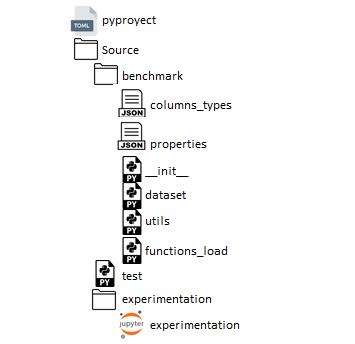
\includegraphics[width=0.5\textwidth]{Graphics/directory.png}
    \caption{Directorio del Benchmark}
    \label{fig:image1}
 \end{figure}

\subsection{Clases de HAutoML-Bench}\label{subsection:class}

\textit{HAutoML-Bench} está formado por dos clases principales  \textit{HAutoMLBench} y \textit{Dataset}.
La clase \textit{HAutoMLBench} es la encargada de interactuar con el usuario, en ella se encuentran todos los 
métodos que permiten probar los sistemas. Estos métodos son estáticos para evitar crear instancias distintas con el fin de acceder
al estado del benchmark y sus funcionalidades. En la subsección \ref{subsection:methods} se discuten cada uno de ellos. 

La clase \textit{Dataset} por otro lado se encarga de modelar cada uno de los conjuntos que pertenecen al benchmark y 
almacena sus propiedades. Las propiedades de un dataset son el nombre, url utilizada para la descarga de su 
contenido, informaciones de la naturaleza de sus datos y una función de carga o llamada 
\textit{loader\_function}. Esta función es la que permite acceder a su contenido. 
Esta clase hereda de la clase \textit{YamlAble}. Esto le brinda la posibilidad  de serializarse como un objeto \textit{.yaml}, 
permitiendo guardar cada uno de sus valores y acceder a ellos de forma rápida y fácil. 

\begin{flushleft} 
    { \textbf{Estructura de las propiedades de un Dataset}}\label{class:dataset_pro}
\end{flushleft}
Las propiedades en los dataset permiten almacenar información relevante para su utilización. El nombre, la url y su función de carga posibilitan acceder a su contenido.
La información sobre sus metadatos permite identificar la complejidad de la tarea que resuelve.
Estos metadatos contienen el número de columnas, el número de instancias de sus partes: entrenamiento y prueba. También la tarea que resuelven y el número de 
valores null que poseen. Además, se brinda para cada conjunto el tipo semántico inferido para cada una de sus columnas. Esta inferencia se realiza a partir de la 
interpretación de la descripción del dataset original. El nombre de la etiqueta de salida es otro de los metadatos, para el dataset \textit{google-guest} se guarda una 
lista ya que posee varias etiquetas que pueden utilizarse como salida. 

En las tareas de clasificación se tiene una lista con los distintos valores de la etiqueta a predecir. En la binaria se tiene una propiedad \textit{positive\_class} 
que indica la clase positva. Por último se tiene un metadato para el número de clases en la tareas de clasificación y el balance de las mismas. 
El balance se mide por el número de instancias de la clase minoritaria frente a la mayoritaria. 
Para más referencia a la estructura de las propiedades ver figura\ref{code:dataset}:      

\begin{lstlisting}[caption= Clase Dataset, label = code:dataset]
class Dataset:
    url: str
    name: str
    loader_function : function
    info : dict = {'n_instances': list[int],
                    'n_columns': int , 
                    'columns_types': dict{'name' : type},
                    'targets': list[str] or str,
                    'null_values': int,
                    'task': str 
                    'positive_class': Any,
                    'class_labels': list[Any] 
                    'n_classes': int, 
                    'class_balance':float}
  
\end{lstlisting}

\begin{flushleft} 
    { \textbf{Tipos semánticos}}\label{class:semantic_types}
\end{flushleft}
Los tipos semánticos de cada columna aportan información sobre el dominio al que pertencen los datos. El brindarlos como información garantiza que el conjunto 
es procesado respetando el significado de cada una de las entradas. Estos se dividen atendiendo a los diferentes tipo de datos y 
se agregan unas clasificaciones especiales para ayudar a entender aun más el problema.

\begin{itemize}
    \item Entradas de texto
    \begin{itemize}
        \item text: Posee más de una idea. Estas pueden o no tener relación.
        \item sentence: Es un texto que transmite una idea esencial. Esta para su entendimiento no puede ser separada en partes.
        \item word: Tiene significado propio es la más pequeña entidad.
        \item syntagma: Es considerado una estructura más compleja que word ya que puede incluir varias de estas. Es una frase 
        que debe procesarse de forma conjunta porque pierde su significado. Esta no indica acción ni estado por tanto no se considera oración. 
    \end{itemize}      
    
    \item Entradas numéricas
    \begin{itemize}
        \item int: número entero.
        \item float: número decimal.
    \end{itemize}

    \item Entradas categóricas
    \begin{itemize}
        \item category: La variable define tipos o categorías.
    \end{itemize}
    
    \item Entradas booleanas
    \begin{itemize}
        \item boolean: Se toman como variables booleanas aquellas que tienen valores True o False.
    \end{itemize}
    
    \item Entradas de Tiempo
    \begin{itemize}
        \item datetime: Columnas que especifican una fecha o un tiempo.
    \end{itemize}
    
    \item Entradas Imagen
    \begin{itemize}
        \item image: Una entidad imagen.
        \item path\_image: La dirección a una carpeta de imágenes.
    \end{itemize}


    \item Entradas Especiales
    \begin{itemize}
        \item SeqTokens: Una lista de palabras a etiquetar como entidad.
        \item SeqLabels: Una lista de etiquetas que corresponden al formato IOB2. 
    \end{itemize}
\end{itemize}

Muchos sistemas son incapacez de tratar con todos estos tipos semánticos o muchos trabajan con los tipo concreto.
Los que sean capaces de tratar con los mismos o con similares, solo necesitan realizar la traducción, sin necesidad de cambiar
la estructura del dataset ya que su estructura y sus tipos son independiente.

\begin{flushleft} 
    { \textbf{Función de carga de cada Dataset: \textit{loader\_function}}}\label{class:loader-function}
\end{flushleft}
La clase \textit{Dataset} posee un metodo para descargar, abrir y leer el contenido propio de cada una de sus instancias.
Este metodo es abstracto por lo que cada conjunto de datos debe realizar su propia implementacion para realizar las tareas antes descritas. 

En el caso de los conjuntos ya pertenecientes al benchamrk sus implementaciones poseen ciertos parámetros de entrada para describir las características del 
contenido que retornan. Es posible especificar el formato de salida del contenido mediante el parámetro \textit{format} este corresponde con el tipo lista o 
dataframe de pandas. 
El parámetro \textit{samples} indica si el conjunto se divide en dos: entrenamiento y prueba o se retorna completo. 
También es posible separar la columna de salida de las de entrada mediante el parámetro booleano \textit{in\_x\_y}. 
Cada conjunto conoce su etiqueta a predecir. El conjunto \textit{google-guest} posee otras que pueden utilizarse como salida por lo que su m'etodo admite un 
parámetro \textit{target}.  

Consultar la figura: \ref{code:loader-function} para obtener más información respecto a la estructura de la función. 

\begin{lstlisting}[caption=Estructura de las fuciones de carga de los dataset, label = code:loader-function]
def function_loader(self, format = "pandas", in_x_y = False ,samples =  2)
    '''
    input: self: Dataset
        format: str
        in_x_y : bool
        samples : int
        target: str only when dataset matches google-guest
    output: tuple	   
        if in_x_y = True, samples = 2  return X_train, y_train ,X_test, y_test
        in_x_y = True, samples = 1 return X_all, y_all
        in_x_y = False, samples = 2  return train, test
        format = "pandas", in_x_y = False, samples =  1  return all
            format:
            pandas : table 
            list : list [[intance1],[intance2]....]
    '''
    \end{lstlisting}


\subsection{Métodos de interacción del usuario}\label{subsection:methods}

\begin{flushleft} 
    { \textbf{ Método \textit{init}}}\label{method:create}
\end{flushleft}
El método \textit{init} inicializa el benchamrk. Para ello almacena en archivos los nombres, urls, las informaciones y los nombres de las funciones de carga de todos 
los dataset que posee. las informaciones están previamente guardadas. 
Luego construye y serializa las intancias de los conjuntos para su uso futuro. Es importante que este método solo se ejecute una sola vez, debido a que los cambios 
que se realicen se perderán. El benchmark vuelve a su estado inicial por defecto, con sus conjuntos originales.

Este no recibe parámetros de entrada ni retorna nigún valor. Cualquier error es reportado en pantalla.

\begin{flushleft} 
    { \textbf{Método \textit{get\_dataset}}}\label{method:get-dataset}
\end{flushleft}

Una vez se inicializa el benchamrk para evaluar los sistemas se debe tener acceso a los conjuntos de datos.
El método \textit{get\_dataset} a partir de un nombre obtiene la instancia de ese dataset almacenado.
A tener la instancia se puede acceder a cada una de sus propiedades, su nombre, sus metadatos, url y su 
función de carga.  
Consultar la figura: \ref{code:get-dataset} para obtener más información respecto a la estructura del método. 



\begin{lstlisting}[caption= Método init,label = code:get-dataset]
def get_dataset(name):
    '''
    Input: name: str 
    Output: dataset : Dataset
    ''' 
\end{lstlisting}
  
\begin{flushleft} 
    { \textbf{Método \textit{add\_dataset} }}\label{method:new}
\end{flushleft}
El método \textit{add\_dataset} agrega un nuevo dataset al benchmark. 
Recibe como entrada el nombre, la url, la función de carga y su parámetro opcional los metadatos.
Si se introducen los metadatos estos pasan por un proceso de verificación con el fin de validar que se introduzcan correctamente.
Sus campos son obligatorios sino se tiene información respecto a uno se deben marcar como \textit{None}.
Se debe tener en cuenta que si existe un conjunto con el mismo nombre se remplazará.

La estructura de los datos de entrada y salida se pueden observar en la figura:\ref{code:add-dataset}. 

\begin{lstlisting}[caption= Método add\_dataset, label= code:add-dataset]
    def add_dataset(cls, name, url, function, metadata = None ):
        '''
        Input:
            name: str
            url: str
            function : function
            metadata : dict{'n_instances': list[int],
                            'n_columns': int , 
                            'columns_types': dict{'name': type},
                            'targets': list[str] or str,
                            'null_values': int,
                            'task': str 
                            'positive_class': Any,
                            'class_labels': list[Any] 
                            'n_classes': int, 
                            'class_balance': float}
        Output: 
        ''' 
\end{lstlisting}

\begin{flushleft} 
    { \textbf{Método \textit{remove\_dataset} }}\label{method:remove}
\end{flushleft}
Este método como su nombre lo indica remueve el dataset que coincida con el nombre que se introduce como parámetro de entrada. 
Produce error en caso de que exista algún problema durante la escritura de los archivos del estado del benchmark.

La figura: \ref{code:remove-dataset} muestra detalles del método.

\begin{lstlisting}[caption= Método remove\_dataset, label= code:remove-dataset]
def remove_dataset(name):
    '''
    input: name: str
    output: None
    '''
\end{lstlisting}

\begin{flushleft} 
    { \textbf{Método \textit{filter}}}\label{method:filter}
\end{flushleft}
El objetivo del método \textit{filter} es devolver una lista de dataset que cumpla con las restricciones de los parámetros de entrada. La primera 
restricción que puede ser introducida es el tipo de tarea. El segundo parámetro es el cumplimiento de una propiedad numérica del 
dataset, esta propiedad debe ser característica de los metadatos. 
En caso de no establecer ninguna restricción se devuelve una lista con todos los dataset introducidos.
Consulte la fig:\ref{code:filter} para ver la estructura de la entrada y salida del método.

\begin{lstlisting}[caption=Método filter, label= code:filter]
def filter(cls, task = None,expresion = None):
    '''
    input:
        task: str = 'binary', 'regression, 'multiclass', 'multiclass'
        expression: tuple(len(3)) = (property,min,max) : min <= property < max
        property: str = 'n_instances','n_columns', 'null_values','n_classes','class_balance'
    output: list[str]
    '''  
\end{lstlisting}

\begin{flushleft} 
    { \textbf{Método \textit{evaluate}}}\label{method:mevaluate}
\end{flushleft}
El método \textit{evaluate} mide el rendimiento de una herramienta de aprendizaje automático. 
Posee parámetros obligatorios como el nombre del conjunto, la lista de valores verdaderos de la salida y los valores que fueron predecidos.
Ambas secuencias deben coincidir en tipos y en tamaño. En el caso de que el conjunto pertenezca al benchamrk y que contenga sus metadatos 
correctamente etiquetados se puede prescindir de introducir los parámetros opcionales. 
Los parámetros opcionales corresponden a la tarea que se pretende evaluar. Además los distintos valores de la etiqueta de salida. Este es necesario para evaluar 
tareas de clasificación multiclase. Otro parámetro opcional es la etiqueta de la clase positiva, es necesaria para clasificaciones binarias y cuando la salida tiene 
valores no numéricos. 
Los últimos parámetros coinciden con el nombre del archivo y la ruta en donde se quieren guardar los resultados. 

El método utiliza las métricas implementadas en el paquete de python \textit{sklearn}. Según el tipo de tarea se evalúan sus métricas correspondientes.
Para las métricas de entidades y relaciones se provee una Implementación de la \textit{precisión}, \textit{recobrado} y \textit{f1\_beta}. 

La salida incluye cada una de las métricas y el valor obtenido para cada una de ellas. Durante la ejecución se escribe un archivo \textit{json} con los resultados 
obtenidos. Este archivo es capaz de almacenar todos los resultados de un sistema en todos los dataset.

La figura muestra la estructura de la entrada y la salida del método \textit{evaluate} fig:\ref{code:evaluate} y la estructura del archivo que almacena los resultados 
experimentales fig: \ref{code:archive-result}.


\begin{lstlisting}[caption=Método evaluate, label= code:evaluate]
    def evaluate( cls, name, y_true, y_pred, is_multilabel = False, task =None, positive_class = None , class_labels = None, save_path = None, name_archive ='results'):
    '''
    input: name: str
           y_true: array, list
           y_pred: array, list
           Non-mandatory parameters input:
           task: str
           positive_class: str
           class_labels: list[str]
           save_path: str : path
           name_archive: str
           output: 
           result: {key: name_metric,value: value_metric}
           '''
        \end{lstlisting}
        
\begin{lstlisting}[caption= Estructura del archivo que almacena los resultados experimentales, label= code:archive-result]
dict{key: name_datasets, value: {key: name_metric,value: value_metric}}
\end{lstlisting}
\begin{flushleft} 
    {\large {\textbf{Métodos de Auxiliares}}}\label{method:methods}
\end{flushleft}
En el archivo \textit{utils.py} se tienen los métodos auxiliares que se encargan de definir las tareas de la clase \textit{Dataset}. Ejemplo de estas funcionalidades 
son la capacidad de serializarse y el proceso inverso. El archivo también guarda métodos que ayudan a la clase \textit{HAutoMLBench}, aquí se almacenan los métodos de 
inicialización y cambio de sus variables de estado: nombres de los conjuntos que pertenecen , sus url, los nombres de sus funciones de carga y sus metadatos.   





